\documentclass[a4paper]{article}
%\documentclass[a4paper]{scrartcl}

\usepackage{url}
\usepackage{amsfonts}
\usepackage{amsmath}
\usepackage{amssymb}
\usepackage{subcaption}
\usepackage{float}
\usepackage{comment}
\usepackage{graphicx}
\usepackage{xcolor}

\renewcommand{\i}[1]{\textit{#1}}

\newcommand\blue[1]{\textcolor{blue}{#1}}


\author{kwxm}
\date{December 2018}
\title{Some benchmarks for transformations of the CEK machine}
\begin{document}
\maketitle

\section*{Introduction}

\noindent This document contains some timing results for various
versions of the CEK machine.  If you look at the description of the
CEK machine you can see that the \texttt{return} phase is essentially
calling a sort of concretised continuation, so I wondered if things
would be any faster with real continuations (short answer: no).

\section*{Experiments}
\noindent I used the following abstract machines.

\begin{itemize}
\item Three versions of the CEK machine from commit \texttt{96fb387}
  (pretty much the earliest version), but with the bounds check for
  sized integers in \texttt{Constant/Make.hs} updated to use the
  \texttt{bit} function rather than calculating $2^n$ for large $n$
  (this was slowing things down quite substantially and has been fixed
  in more recent versions).
\begin{itemize}
\item The original CEK machine
\item The CEK machine with a refunctionalisation transformation
  applied so that it uses explicit continuations rather than
  the frames and \texttt{return} operation in the contextual version
  of the CEK machine.
\item The refunctionalised version with an ``un-CPS'' transformation
  applied.  This essentially turns the machine into a simple recursive
  evaluator providing a direct implementation of a standard structural
  operational semantics.
\end{itemize}
\item The current CEK machine at commit \texttt{c9a8ae24}.  This has been
  significantly modified from the earlier version, using monads and
  including the new infrastructure for ``dynamic'' built-in functions.
\end{itemize}

\noindent Olivier Danvy and a number of collaborators have done a lot
of work on transformations of abstract machines (see ``A Functional
Correspondence between Evaluators and Abstract Machines'', for
example), and the transformations here are instances of the kind of
thing they've studied.
\\

\subsection*{Inputs}
The programs were run with the inputs shown in
Figure~\ref{fig:benchmark-inputs}. These are the same (hand-written)
programs and inputs as were used for evaluation of the lazy machine in
a previous document, and the same statistics were used (collected using
\texttt{/usr/bin/time -f "\%U \%S \%M"} on Linux). The programs are all
recursive programs using the $Z$ combinator:

\begin{itemize}
\item \texttt{Loop}: loop $n$ times.
\item \texttt{Tri}: calculate $n + (n-1) + \ldots + 2 + 1$
\item \texttt{Fac}: calculate $n(n-1)\cdots2\cdot1$ (requires very large integers)
\item \texttt{Fib}: Naive recursive Fibonacci
  \end{itemize}




The programs were
run once only for each input;  ideally we'd run them several times
each and take the average, but this would be a lengthy process and
the results below don't suggest that we'd gain much from a more detailed
test.

\begin{figure}[H]
\centering
\begin{tabular}{|l|r|r|r|r|} 
\hline
Program   & Minimum input & Step & Maximum input & Integer size (bytes) \\
\hline
\texttt{Loop} & 0 & 20,000 & 1,000,000 & 4\\
\texttt{Tri}  & 0 & 50,000 & 2,000,000 & 8\\
\texttt{Fac}  & 0 & 5,000 & 100,000 & 190,000\\
\texttt{Fib}  & 1 & 1 & 31 & 4 \\
\hline
\end{tabular}
\caption{Programs and inputs}\label{fig:benchmark-inputs}
\end{figure}


\newpage
\section*{Results}
\begin{figure}[H]
\centering 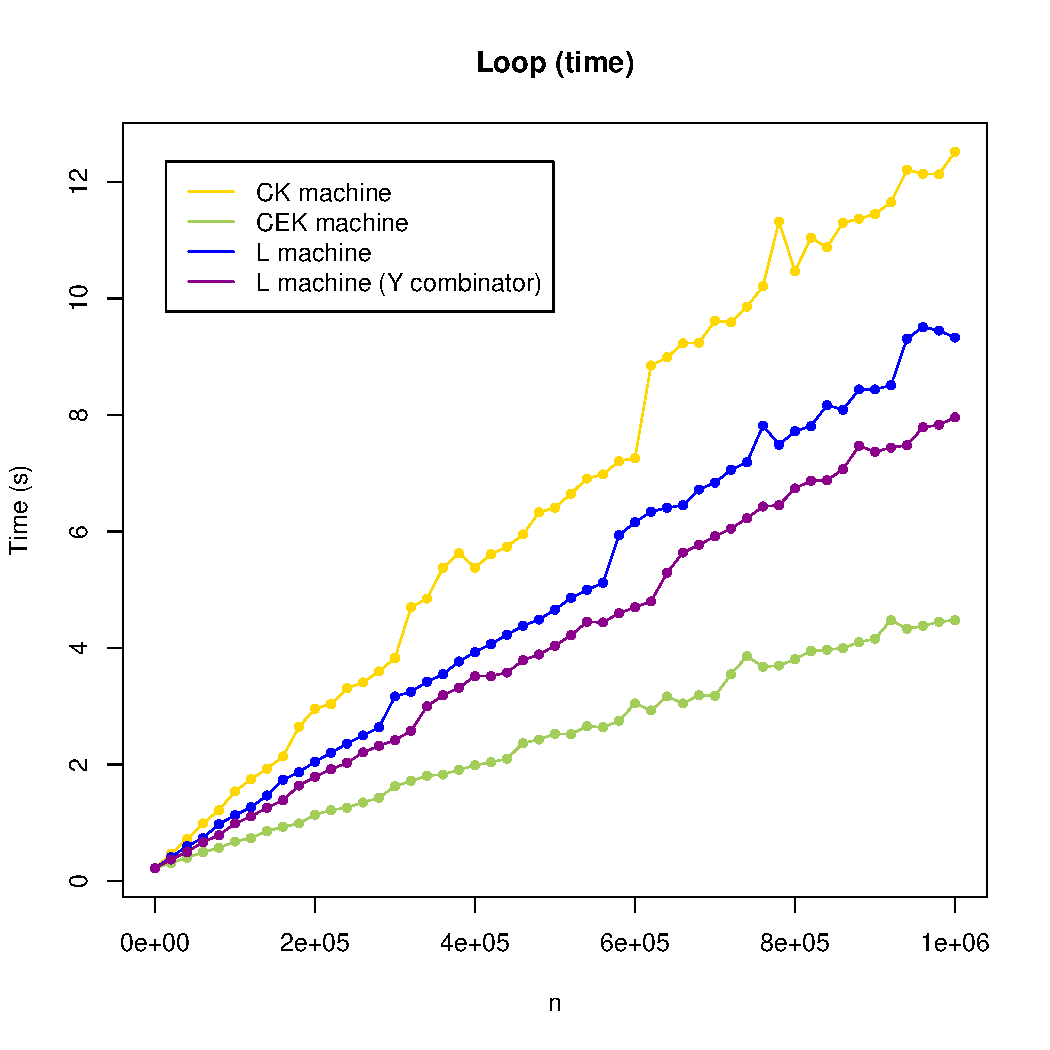
\includegraphics[width=0.8\linewidth]{loop-times.pdf}

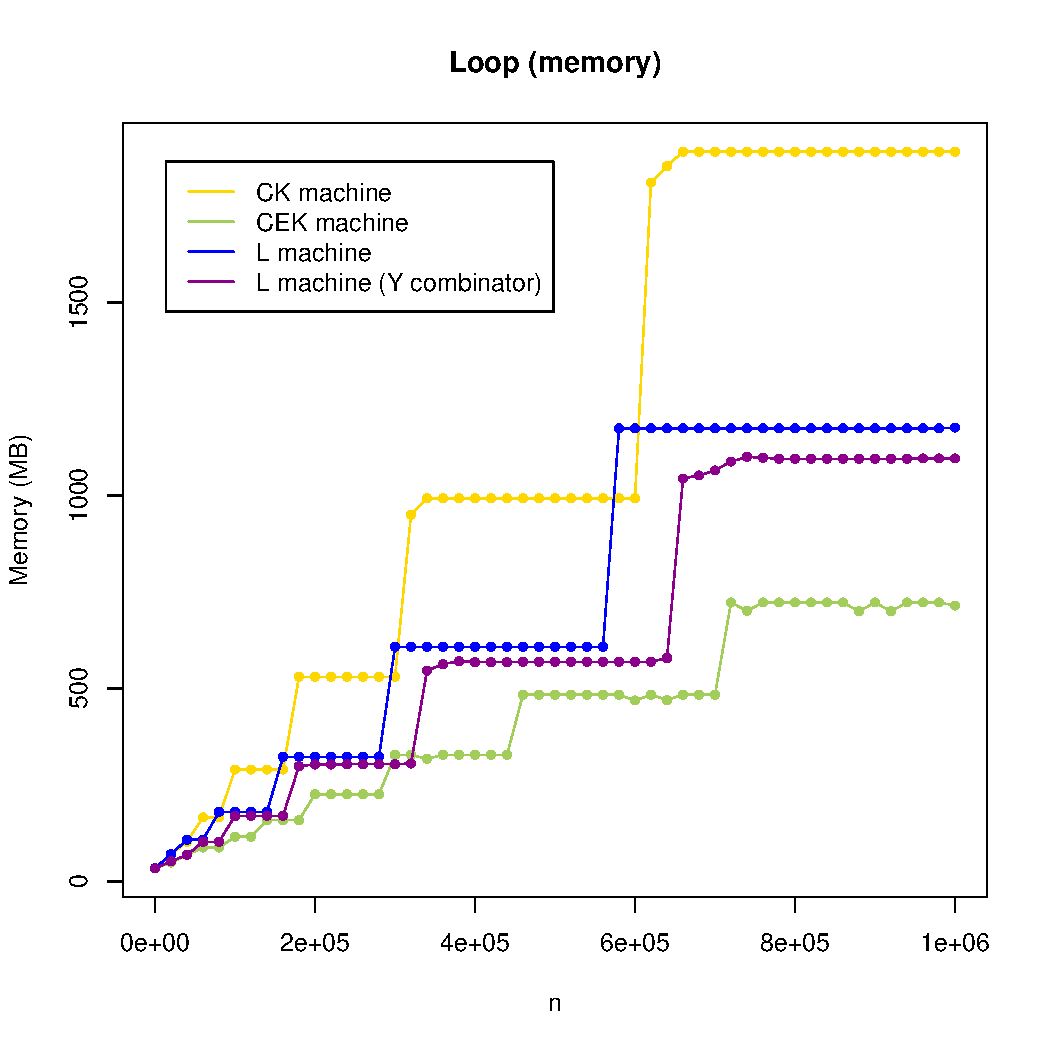
\includegraphics[width=0.8\linewidth]{loop-mem.pdf}
\caption{Loop}\label{fig:loop-graphs}
\end{figure}
\newpage

\begin{figure}[H]
\centering
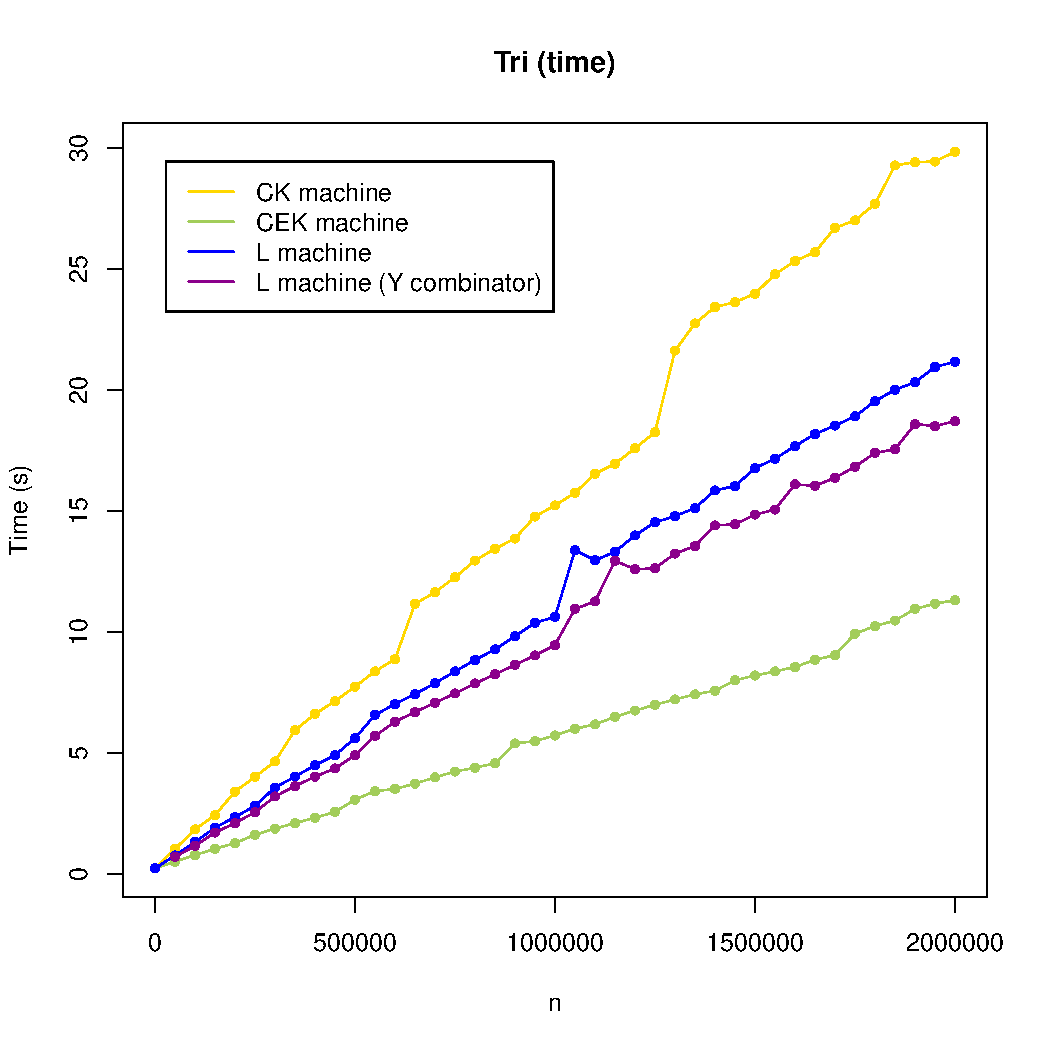
\includegraphics[width=0.8\linewidth]{tri-times.pdf}

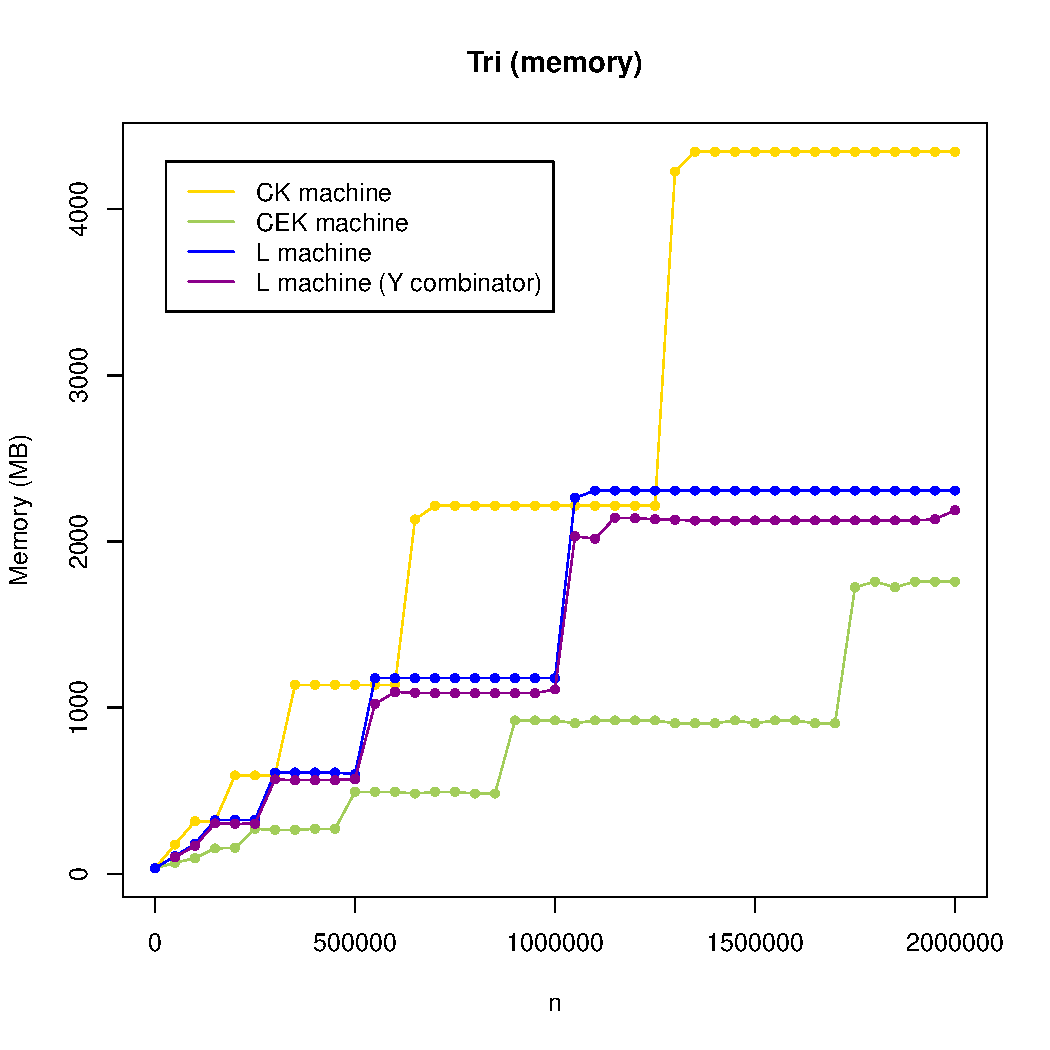
\includegraphics[width=0.8\linewidth]{tri-mem.pdf}
\caption{Triangular numbers}\label{fig:tri-graphs}
\end{figure}
\newpage

\begin{figure}[H]
\centering
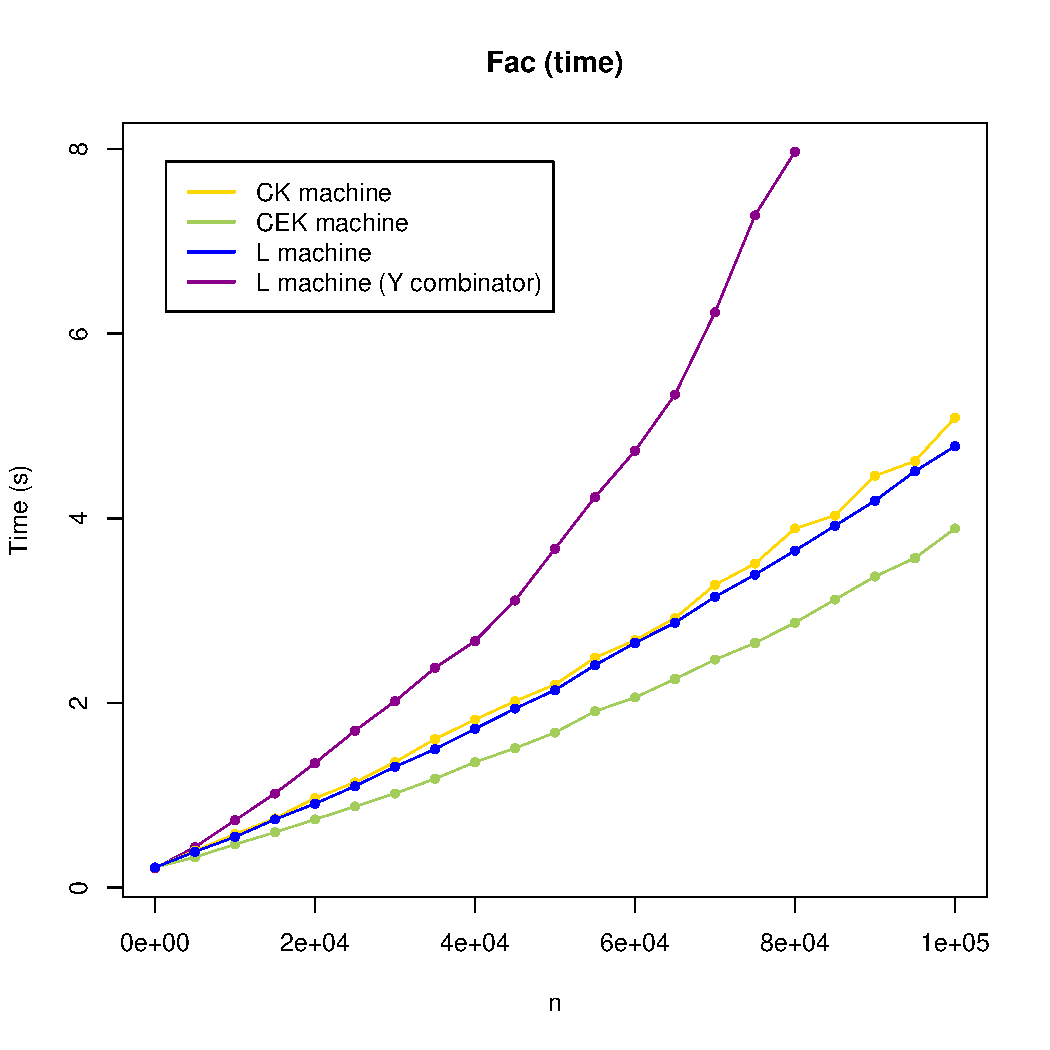
\includegraphics[width=0.8\linewidth]{fac-times.pdf}
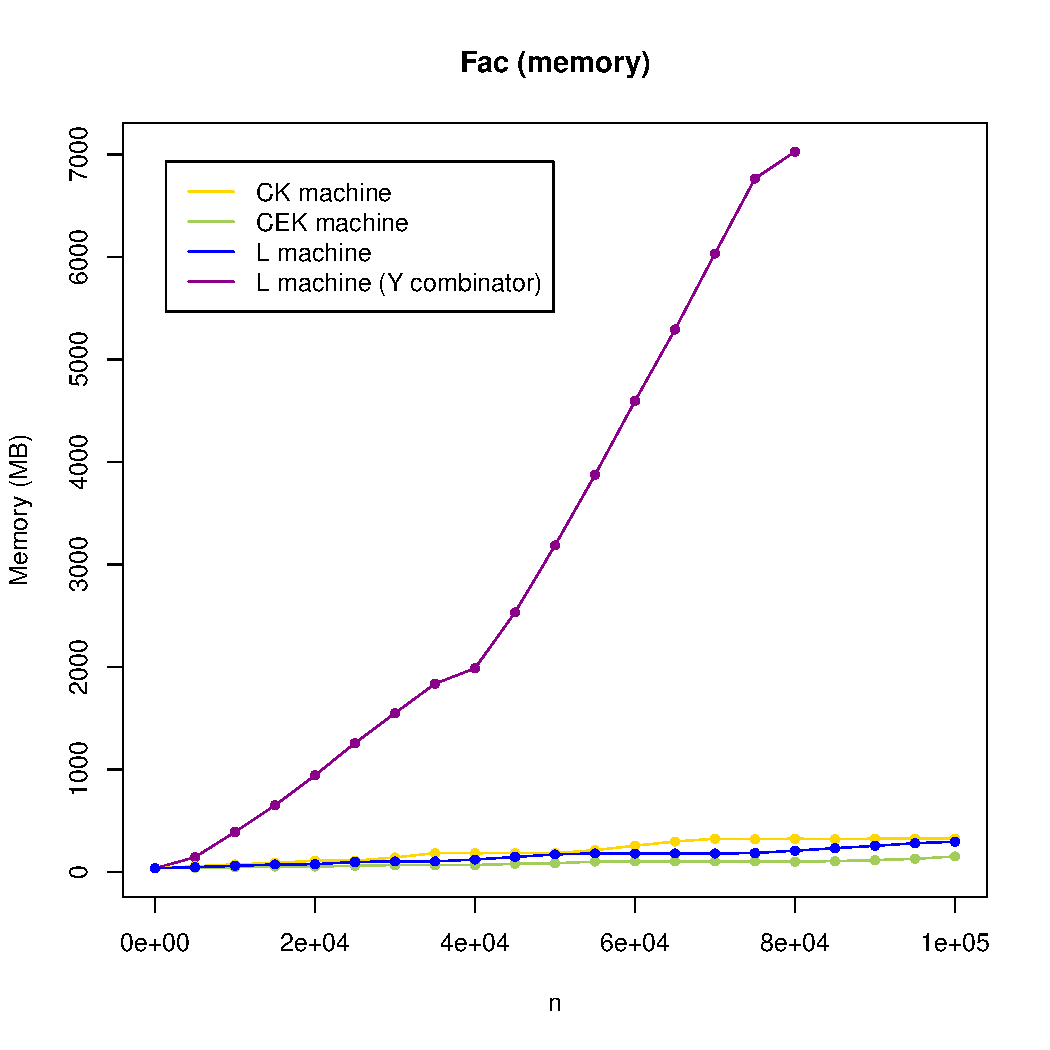
\includegraphics[width=0.8\linewidth]{fac-mem.pdf}
\caption{Factorial}\label{fig:fac-graphs}
\end{figure}

\newpage
\begin{figure}[H]
\centering
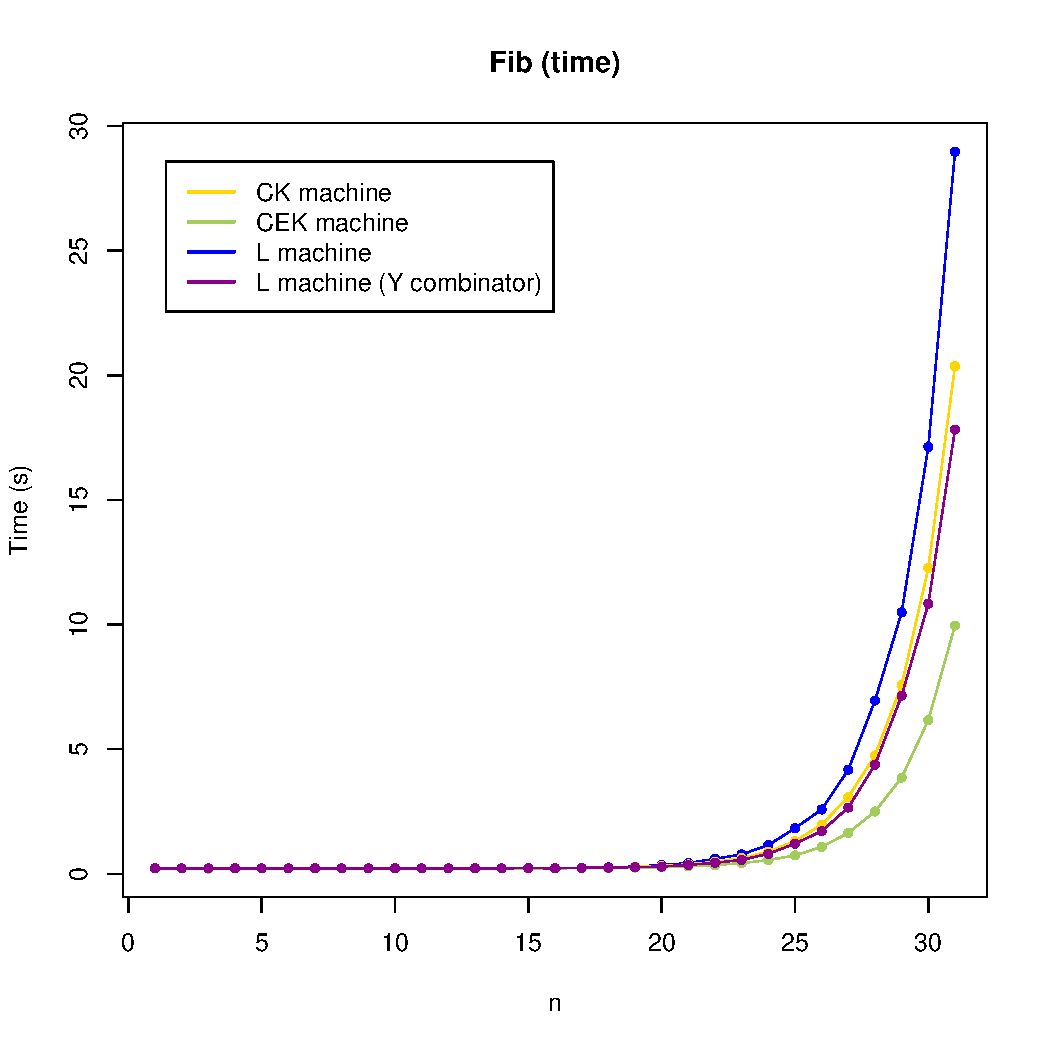
\includegraphics[width=0.8\linewidth]{fib-times.pdf}
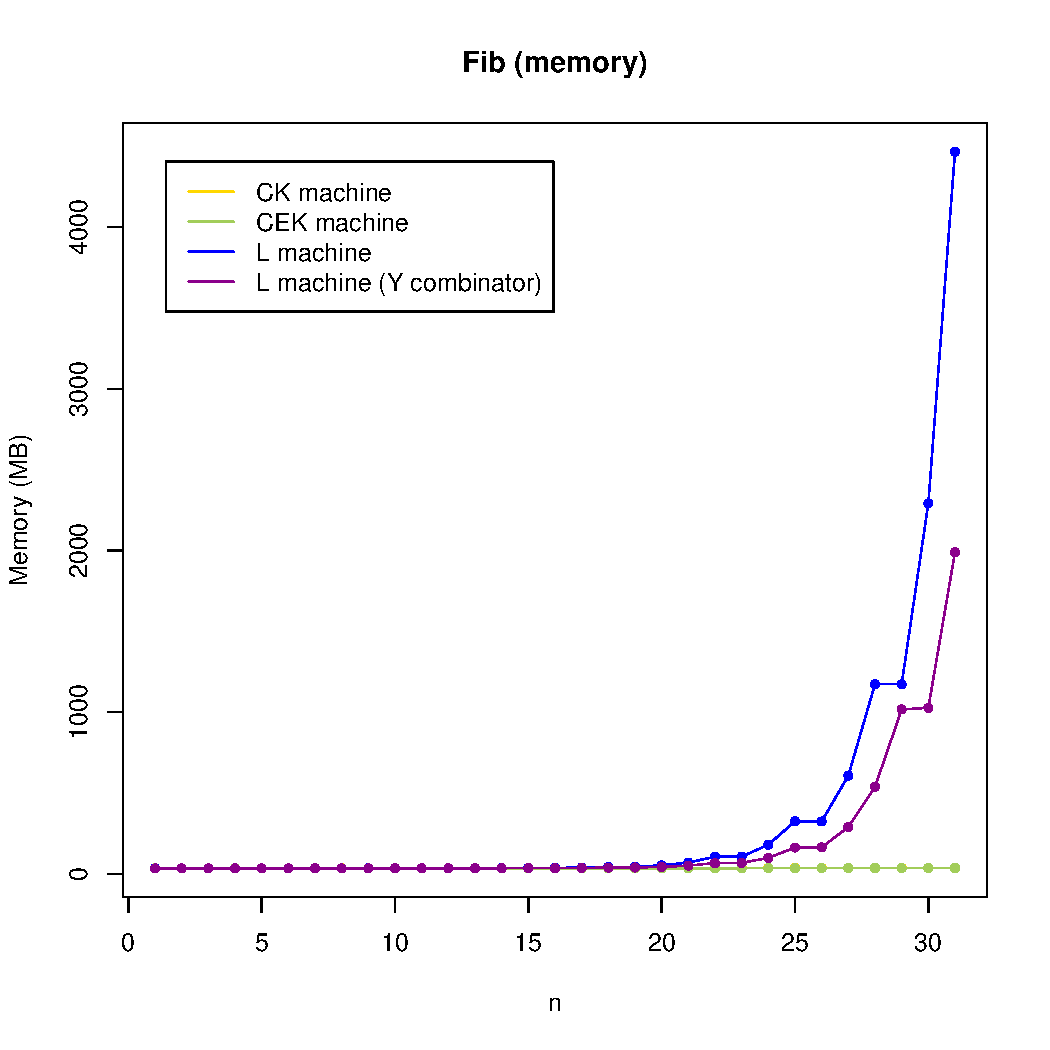
\includegraphics[width=0.8\linewidth]{fib-mem.pdf}
\caption{Fibonacci}\label{fig:fib-graphs}
\end{figure}

\newpage
\section*{Conclusions}
The results are pretty inconclusive: the variations on the original
CEK machine don't seem to make a lot of difference, possibly because
GHC will be transforming things behind the scenes anyway.

It's notable that the current version of the CEK machine is quite a
bit slower than the original one in some cases.  This is presumably
because it's quite a bit more complicated now, and also partly because
there's at least one problem (to do with renaming variables in
booleans) which we've identified but which I don't think has been
fixed in the master branch yet.

It's also the case that the memory usage of the current version is
significantly lower than the old version in some cases: I have no idea
why this is.  We should do some detailed profiling on complicated
examples.


\end{document}
